\documentclass{article}
\usepackage{iclr2026_conference,times}
\input{math_commands.tex}

\usepackage{hyperref}
\usepackage{url}
\usepackage{booktabs}
\usepackage{graphicx}
\usepackage{amsmath}
\usepackage{amssymb}
\usepackage{multirow}
\usepackage{xcolor}
\usepackage{subcaption}
\usepackage{algorithm}
\usepackage{algorithmic}
\usepackage{colortbl}
\usepackage{enumitem}
\usepackage{array}
\usepackage{makecell}

% Custom commands
\newcommand{\bench}{\textsc{ConsistencyBench}}
\newcommand{\method}{\textsc{CGD}}
\newcommand{\ia}{\text{IA}}
\newcommand{\pcr}{\text{PCR}}
\newcommand{\scr}{\text{SCR}}

\title{Logical Consistency Under Pressure: \\Probing and Repairing Cross-Query Contradictions in LLMs}

\author{Anonymous}

\newcommand{\fix}{\marginpar{FIX}}
\newcommand{\new}{\marginpar{NEW}}

\begin{document}
\maketitle

\begin{abstract}
Large language models answer individual logic questions with reasonable accuracy, yet frequently contradict themselves across logically related queries, affirming a conditional while denying its contrapositive, or endorsing a transitive chain while rejecting the implied conclusion. We introduce \bench{}, a benchmark of 493 logically entailed question sets (1,904 questions) spanning six categories of formal and commonsense reasoning, designed to measure \emph{cross-query logical consistency}. We evaluate eighteen frontier LLMs, including GPT-5.2, GPT-4.1, Claude Opus~4.6, Gemini~2.5 Pro, DeepSeek-R1, o3, and Qwen~2.5 72B, and find that even the strongest model (GPT-4.1) achieves only 46.7\% set-level consistency despite 83.0\% individual accuracy, revealing consistency gaps of \textbf{36--57 percentage points} across all models tested. We propose \emph{Consistency-Guided Decoding} (\method{}), a training-free, model-agnostic inference-time method that detects and repairs cross-query contradictions via NLI-based checking. Across 17 models, \method{} improves set-level consistency by \textbf{+6.6pp} on average (up to \textbf{+19.7pp} for GPT-4o), while simultaneously improving individual accuracy by +2.8pp on average, demonstrating that cross-query consistency is a tractable target for inference-time intervention.
\end{abstract}

% ============================================================
\section{Introduction}
\label{sec:intro}
% ============================================================

Logical reasoning is fundamental to reliable AI systems. Real-world reasoning requires not just answering individual questions correctly, but maintaining \emph{logical coherence across related inferences}. A physician who diagnoses hypertension but denies the patient has elevated blood pressure has failed not on knowledge but on consistency. Similarly, an LLM-powered legal assistant that affirms ``if the contract is breached, damages are owed'' but denies ``since damages are not owed, the contract was not breached'' makes logically contradictory claims despite both questions arising from the same premise.

Large language models (LLMs) have achieved impressive reasoning performance on isolated benchmarks \citep{wei2022chain, wang2023selfconsistency, openai2024o1}, yet their cross-query consistency remains poorly understood. The ``reversal curse'' \citep{berglund2023reversal} demonstrated that models trained on ``A is B'' fail to generalize to ``B is A.'' We show that this problem extends far beyond pairwise reversal: LLMs \emph{systematically} contradict themselves across diverse logical relationships including contrapositive equivalence, transitivity, syllogistic reasoning, negation, modus tollens, and commonsense entailment (Figure~\ref{fig:overview}).

\begin{figure*}[t]
\centering
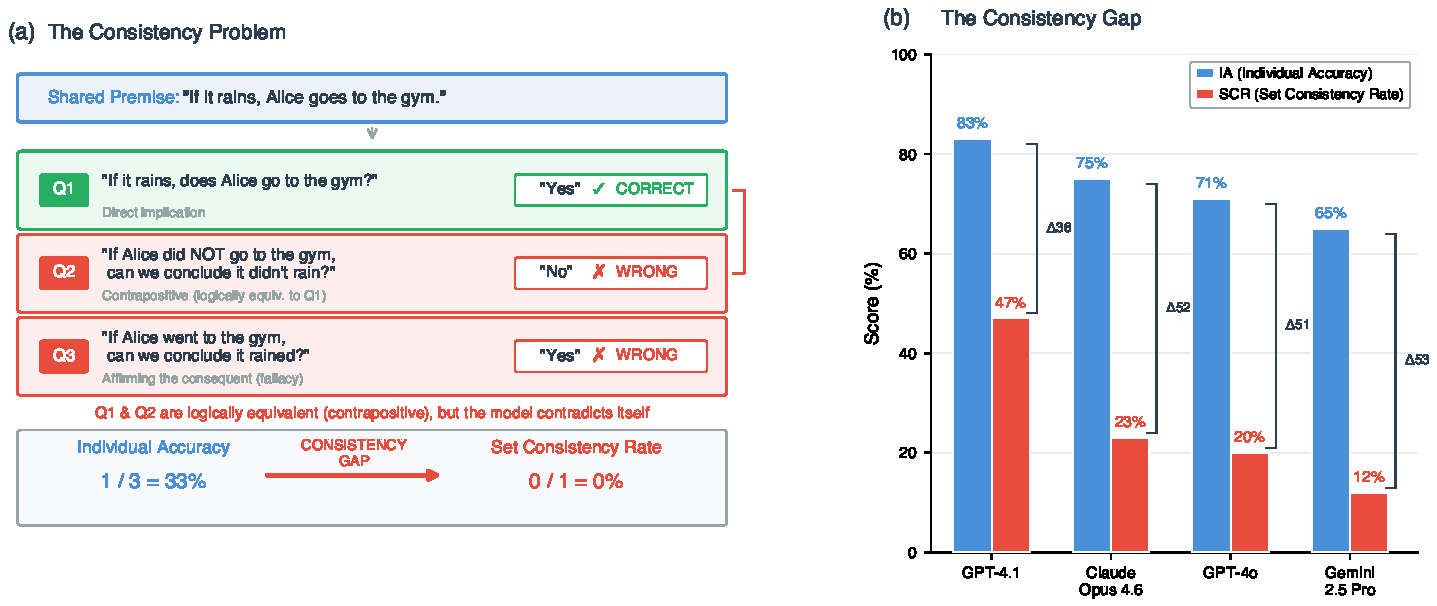
\includegraphics[width=\textwidth]{figures/figure1_overview.pdf}
\caption{\textbf{The cross-query consistency problem.} \textbf{(a)} A model correctly answers Q1 (direct implication) but contradicts itself on Q2 (the logically equivalent contrapositive) and incorrectly affirms Q3 (the invalid ``affirming the consequent'' fallacy). Despite 33\% individual accuracy, the set-level consistency rate is 0\%. \textbf{(b)} The consistency gap across four representative models: individual accuracy (IA) far exceeds set-level consistency (SCR), with gaps of 36--53 percentage points.}
\label{fig:overview}
\end{figure*}

We make three contributions: \textbf{(1)} \bench{}, a benchmark of 493 question sets (1,904 questions) spanning six logical reasoning categories, with three hierarchical consistency metrics (\S\ref{sec:benchmark}); \textbf{(2)} a systematic evaluation of 18 frontier LLMs revealing that all models exhibit consistency gaps of 36--57 percentage points between individual accuracy and set-level consistency, a finding that holds across model families, scales, and training paradigms including reasoning-specialized models (\S\ref{sec:experiments}); and \textbf{(3)} Consistency-Guided Decoding (\method{}), a training-free, model-agnostic inference-time method that improves consistency in 16 out of 17 models tested, with a mean improvement of +6.6pp and a maximum of +19.7pp (\S\ref{sec:method}).

% ============================================================
\section{Related Work}
\label{sec:related}
% ============================================================

\paragraph{LLM Logical Reasoning.}
Recent benchmarks evaluate LLMs on propositional logic \citep{saparov2023language}, first-order logic \citep{han2022folio}, and syllogistic reasoning \citep{dasgupta2022language}, but focus on single-query accuracy. These benchmarks measure whether a model can answer a logic question correctly in isolation. We measure a complementary and distinct property: \emph{whether a model maintains consistency across logically related queries derived from the same premises}.

\paragraph{Consistency Failures.}
\citet{berglund2023reversal} exposed the reversal curse, showing that training on ``A is B'' does not yield ``B is A.'' \citet{raj2023semantic} studied semantic consistency under paraphrasing, measuring whether models give equivalent answers to rephrased questions. \citet{shi2023large} showed sensitivity to irrelevant context. Our work extends the consistency analysis to multi-step logical relationships at scale, testing six distinct categories of logical entailment across 18 models.

\paragraph{Inference-Time Reasoning.}
Chain-of-thought prompting \citep{wei2022chain} and self-consistency decoding \citep{wang2023selfconsistency} improve single-query accuracy but do not enforce cross-query coherence, since each question is processed independently. Maieutic prompting \citep{jung2022maieutic} detects self-contradictions within a single response but requires expensive abductive/deductive candidate generation. Neuro-symbolic approaches \citep{pan2023logic, xu2024symbcot} require structured formal representations. In contrast, \method{} operates entirely in natural language, is training-free, and works with black-box APIs without access to model internals.

% ============================================================
\section{\bench{}: A Benchmark for Cross-Query Logical Consistency}
\label{sec:benchmark}
% ============================================================

\bench{} contains 493 question sets comprising 1,904 individual questions across six categories (Table~\ref{tab:categories}). Each set shares a common premise and contains 3--4 questions that test logically related inferences. Ground-truth answers are derived from classical propositional and first-order logic for the formal categories and from manually curated entailment rules for commonsense reasoning. Questions are generated programmatically from curated pools of 24 person names, 20 factual statements, 10 activity pairs, 8 condition pairs, 10 abstract categories, and 70 commonsense entailment rules, ensuring diversity while maintaining logical soundness.

\begin{table}[t]
\caption{The six categories of \bench{}. Each category tests a specific logical pattern and includes a question designed to detect a common fallacy.}
\label{tab:categories}
\vspace{-0.5em}
\begin{center}
\small
\begin{tabular}{llcl}
\toprule
\textbf{Category} & \textbf{Pattern} & \textbf{\#Sets} & \textbf{Fallacy Tested} \\
\midrule
Contrapositive & $P{\to}Q \equiv \neg Q{\to}\neg P$ & 85 & Affirm.\ consequent \\
Transitivity & $A{\to}B, B{\to}C \vdash A{\to}C$ & 85 & Chain break \\
Syllogistic & $\forall x: A(x){\to}B(x)$ & 85 & Converse error \\
Negation & $P$ vs.\ $\neg P$ & 85 & Neg.\ incoherence \\
Modus Tollens & $P{\to}Q, \neg Q \vdash \neg P$ & 85 & Deny antecedent \\
Commonsense & Everyday entailment & 68 & Reverse entailment \\
\midrule
\textbf{Total} & & \textbf{493} & \\
\bottomrule
\end{tabular}
\end{center}
\vspace{-1em}
\end{table}

\paragraph{Metrics.} We define three hierarchical metrics with increasing strictness. \textbf{Individual Accuracy (IA)} measures the fraction of individual questions answered correctly. \textbf{Pairwise Consistency Rate (PCR)} measures the fraction of within-set question pairs where both are answered correctly. \textbf{Set-Level Consistency Rate (SCR)} measures the fraction of sets where \emph{all} questions are answered correctly. The \emph{consistency gap}, defined as $\text{IA} - \text{SCR}$, quantifies how much single-query accuracy metrics overestimate a model's true logical reasoning capability.

% ============================================================
\section{Consistency-Guided Decoding}
\label{sec:method}
% ============================================================

We propose \method{}, a training-free inference-time method for improving cross-query logical consistency. For each question $q_i$ in a set, \method{} operates in three steps (Algorithm~\ref{alg:cgd}):

\textbf{(1) Generate}: The target LLM $\mathcal{M}$ produces an initial answer $a_i$ for question $q_i$.
\textbf{(2) Check}: An NLI contradiction checker $\mathcal{C}$ (GPT-4o-mini) tests whether $a_i$ contradicts any prior answer $a_j$ in the answer history.
\textbf{(3) Repair}: If a contradiction is detected, a revision prompt that includes the conflicting prior answer $a_j$, the corresponding question $q_j$, and the shared premise is sent to $\mathcal{M}$ to elicit a corrected answer $a_i'$.

\begin{algorithm}[t]
\caption{Consistency-Guided Decoding (\method{})}
\label{alg:cgd}
\begin{algorithmic}[1]
\REQUIRE Question set $\mathcal{Q} = \{q_1, \ldots, q_n\}$, premise $P$, LLM $\mathcal{M}$, NLI checker $\mathcal{C}$
\STATE $\text{history} \leftarrow []$
\FOR{$i = 1$ to $n$}
    \STATE $a_i \leftarrow \mathcal{M}(q_i, P)$ \hfill \COMMENT{Generate}
    \FOR{$(q_j, a_j) \in \text{history}$}
        \IF{$\mathcal{C}(a_j, a_i) = \textsc{Contradiction}$}
            \STATE $a_i \leftarrow \mathcal{M}(\textsc{Revise}(q_i, q_j, a_j, P))$ \hfill \COMMENT{Repair}
            \STATE \textbf{break}
        \ENDIF
    \ENDFOR
    \STATE $\text{history}.\text{append}((q_i, a_i))$
\ENDFOR
\RETURN $\{a_1, \ldots, a_n\}$
\end{algorithmic}
\end{algorithm}

\method{} is model-agnostic (works with any LLM including black-box APIs), training-free (requires no fine-tuning or parameter updates), and efficient (adds at most $O(n)$ NLI checks per question, where $n$ is the set size, typically 3--4). Figure~\ref{fig:cgd} in Appendix~\ref{app:cgd} illustrates the full pipeline.

% ============================================================
\section{Experiments}
\label{sec:experiments}
% ============================================================

\subsection{Setup}

\paragraph{Models.} We evaluate 18 frontier LLMs spanning six model families: \textbf{OpenAI}: GPT-5.2, GPT-5, GPT-5 Mini, GPT-4.1, GPT-4o \citep{openai2024gpt4o}, o3 \citep{openai2025o3, openai2025gpt5}; \textbf{Anthropic}: Claude Opus~4.6, Sonnet~4.6, Sonnet~4.5, 3.5 Sonnet \citep{anthropic2025claude4, anthropic2024claude}; \textbf{Google}: Gemini~2.5 Pro, 2.5 Flash, 2.0 Flash \citep{google2025gemini25, google2024gemini}; \textbf{DeepSeek}: V3.2, R1 \citep{deepseekai2025deepseekv3, deepseekai2025deepseekr1}; \textbf{Meta}: Llama~3.3 70B, 3.1 70B \citep{meta2024llama33, dubey2024llama}; \textbf{Qwen}: 2.5 72B \citep{qwen2024qwen25}. This selection spans multiple scales, architectures, and training paradigms, including reasoning-specialized models (o3, DeepSeek-R1).

\paragraph{Evaluation protocol.} All 18 models are evaluated under \textbf{Direct} (vanilla) prompting with concise yes/no/cannot-determine answers; 17 models under \method{} (DeepSeek-R1 excluded due to API constraints); and 2 models under \textbf{Chain-of-Thought (CoT)} prompting (GPT-4o, Qwen~2.5 72B). Evaluation uses a stratified sample of 300 sets (50 per category, 1,150 questions total).

\subsection{Main Results}

Table~\ref{tab:main} presents the central finding: \emph{every model exhibits a large gap between individual accuracy and set-level consistency}, and \method{} improves SCR for 16 of 17 models tested.

\begin{table}[t]
\caption{Direct prompting vs.\ \method{} on \bench{} (300 sets, 1,150 questions). Gap = IA $-$ SCR. $\Delta$SCR = absolute SCR change with \method{}. Models sorted by vanilla SCR. Best SCR per model in \textbf{bold}. Full per-category results in Appendix~\ref{app:fullcategory}.}
\label{tab:main}
\vspace{-0.5em}
\begin{center}
\scriptsize
\setlength{\tabcolsep}{2.8pt}
\begin{tabular}{l ccc c ccc c}
\toprule
 & \multicolumn{3}{c}{\textbf{Direct}} & & \multicolumn{3}{c}{\textbf{\method{} (Ours)}} & \\
\cmidrule{2-4} \cmidrule{6-8}
\textbf{Model} & \textbf{IA} & \textbf{SCR} & \textbf{Gap} & & \textbf{IA} & \textbf{SCR} & \textbf{Gap} & \textbf{$\Delta$SCR} \\
\midrule
GPT-4.1 & 83.0 & 46.7 & 36.4 & & 85.2 & \textbf{54.0} & 31.2 & +7.3 \\
Qwen 2.5 72B & 75.0 & 32.7 & 42.3 & & 73.7 & \textbf{33.0} & 40.7 & +0.3 \\
Cl.\ Opus 4.6 & 74.8 & 23.3 & 51.4 & & 79.1 & \textbf{32.3} & 46.8 & +9.0 \\
DeepSeek-R1 & 70.2 & \textbf{21.7} & 48.5 & & -- & -- & -- & -- \\
GPT-4o & 70.8 & 20.0 & 50.8 & & 79.0 & \textbf{39.7} & 39.4 & +19.7 \\
Llama 3.1 70B & 65.3 & \textbf{19.0} & 46.3 & & 61.6 & 17.0 & 44.6 & $-$2.0 \\
Gemini 2.5 Flash & 67.6 & 17.7 & 49.9 & & 69.2 & \textbf{22.3} & 46.9 & +4.7 \\
Cl.\ 3.5 Sonnet & 71.6 & 17.3 & 54.2 & & 73.5 & \textbf{22.0} & 51.5 & +4.7 \\
Gemini 2.5 Pro & 65.4 & 12.3 & 53.1 & & 67.7 & \textbf{21.7} & 46.0 & +9.3 \\
GPT-5.2 & 69.3 & 12.0 & 57.3 & & 73.2 & \textbf{23.7} & 49.6 & +11.7 \\
o3 & 67.2 & 12.0 & 55.2 & & 70.3 & \textbf{21.0} & 49.3 & +9.0 \\
Llama 3.3 70B & 56.8 & 10.7 & 46.1 & & 57.0 & \textbf{13.3} & 43.6 & +2.7 \\
Cl.\ Sonnet 4.5 & 51.9 & 10.7 & 41.2 & & 54.7 & \textbf{12.0} & 42.7 & +1.3 \\
Cl.\ Sonnet 4.6 & 57.5 & 10.3 & 47.1 & & 67.0 & \textbf{24.3} & 42.6 & +14.0 \\
DeepSeek V3.2 & 59.2 & 10.0 & 49.2 & & 61.7 & \textbf{19.3} & 42.4 & +9.3 \\
GPT-5 & 62.9 & 9.3 & 53.5 & & 63.6 & \textbf{11.3} & 52.2 & +2.0 \\
Gemini 2.0 Flash & 44.7 & 7.3 & 37.4 & & 55.7 & \textbf{12.3} & 43.4 & +5.0 \\
GPT-5 Mini & 58.4 & 4.0 & 54.4 & & 57.4 & \textbf{9.0} & 48.4 & +5.0 \\
\midrule
\textbf{Mean} & 65.1 & 16.5 & 48.6 & & 67.6 & 22.8 & 44.8 & +6.6 \\
\bottomrule
\end{tabular}
\end{center}
\vspace{-0.5em}
\end{table}

\subsection{Key Findings}

\textbf{(1) The consistency gap is universal.} All 18 models exhibit IA~$>$~SCR, with gaps ranging from 36.4pp (GPT-4.1) to 57.3pp (GPT-5.2). Even the best-performing model, GPT-4.1, achieves only 46.7\% SCR despite 83.0\% IA. The mean gap across all models is 48.6pp, indicating that standard accuracy metrics dramatically overestimate logical reasoning capability.

\textbf{(2) Scaling and reasoning tokens do not solve consistency.} GPT-5.2, one of the newest models, reaches only 12.0\% SCR (gap: 57.3pp). The reasoning-specialized o3 also reaches only 12.0\% SCR despite extended inference-time computation. GPT-5 achieves 9.3\% SCR, and GPT-5 Mini only 4.0\%. These results suggest that scale and reasoning-time compute address different failure modes than cross-query consistency.

\textbf{(3) \method{} works broadly.} Across 17 models, \method{} improves SCR for 16 (94\%), with a mean improvement of +6.6pp and a median of +5.0pp. The largest gains are observed for GPT-4o (+19.7pp), Claude Sonnet~4.6 (+14.0pp), GPT-5.2 (+11.7pp), and Gemini~2.5 Pro (+9.3pp). Only Llama~3.1 70B shows a decrease ($-$2.0pp), suggesting that weaker models may propagate errors through the revision mechanism.

\textbf{(4) \method{} simultaneously improves accuracy.} Beyond consistency, \method{} also improves IA by +2.8pp on average. The contradiction-aware revision process does not merely enforce agreement across answers but helps the model arrive at more correct answers, suggesting that the knowledge needed for consistency is often latent but not reliably activated during independent generation.

\paragraph{Chain-of-Thought comparison.} On GPT-4o, CoT improves IA from 70.8\% to 75.0\% and SCR from 20.0\% to 28.3\%, whereas \method{} achieves 79.0\% IA and 39.7\% SCR. On Qwen~2.5 72B, CoT improves IA from 75.0\% to 77.1\% but \emph{slightly decreases} SCR from 32.7\% to 32.3\%. This confirms that independent reasoning paths, even when they individually improve accuracy, can still be mutually inconsistent. The full strategy comparison is in Appendix~\ref{app:strategies}.

% ============================================================
\section{Discussion and Limitations}
\label{sec:discussion}
% ============================================================

Our results reveal that cross-query logical consistency is a fundamental weakness of current LLMs that is not addressed by scaling, reasoning tokens, or chain-of-thought prompting. The consistency gap persists across all six model families tested, from the latest GPT-5 series to open-weight models like Llama and Qwen, and from general-purpose models to reasoning-specialized ones like o3 and DeepSeek-R1.

\method{} demonstrates that lightweight inference-time intervention can substantially narrow this gap. The approach is practical for deployment: it requires no fine-tuning, works with black-box APIs, and the NLI checker (GPT-4o-mini) adds minimal computational cost. The fact that models can often correct themselves when shown a contradiction suggests that consistency knowledge is encoded in the model's parameters but is not reliably activated during independent generation. This ``latent consistency'' hypothesis points toward promising directions for both training-time and inference-time solutions.

\paragraph{Limitations.} \bench{} covers propositional and first-order logic patterns but does not include temporal, probabilistic, modal, or domain-specific reasoning. \method{} depends on the NLI checker's quality; false positives could degrade performance, as possibly evidenced by the negative result on Llama~3.1 70B ($-$2.0pp). The method adds inference latency proportional to the set size. CoT was evaluated on only 2 of 18 models due to cost constraints. All models are accessed via commercial APIs, and results may vary across API versions or updates.

% ============================================================
\section{Conclusion}
\label{sec:conclusion}
% ============================================================

We presented \bench{}, a benchmark for measuring cross-query logical consistency across six reasoning categories, and \method{}, a training-free inference-time method for improving it. Across 18 frontier LLMs, we found a universal consistency gap of 36--57 percentage points between individual accuracy and set-level consistency. \method{} narrows this gap for 16 of 17 models tested (mean +6.6pp, max +19.7pp) through NLI-based contradiction detection and revision, while simultaneously improving individual accuracy. Our findings demonstrate that cross-query logical consistency is both a significant blind spot in current LLM evaluation and a tractable target for inference-time intervention.

\bibliography{references}
\bibliographystyle{iclr2026_conference}

% ============================================================
% APPENDIX
% ============================================================
\appendix

% ============================================================
\section{CGD Pipeline Diagram}
\label{app:cgd}
% ============================================================

\begin{figure}[ht]
\centering
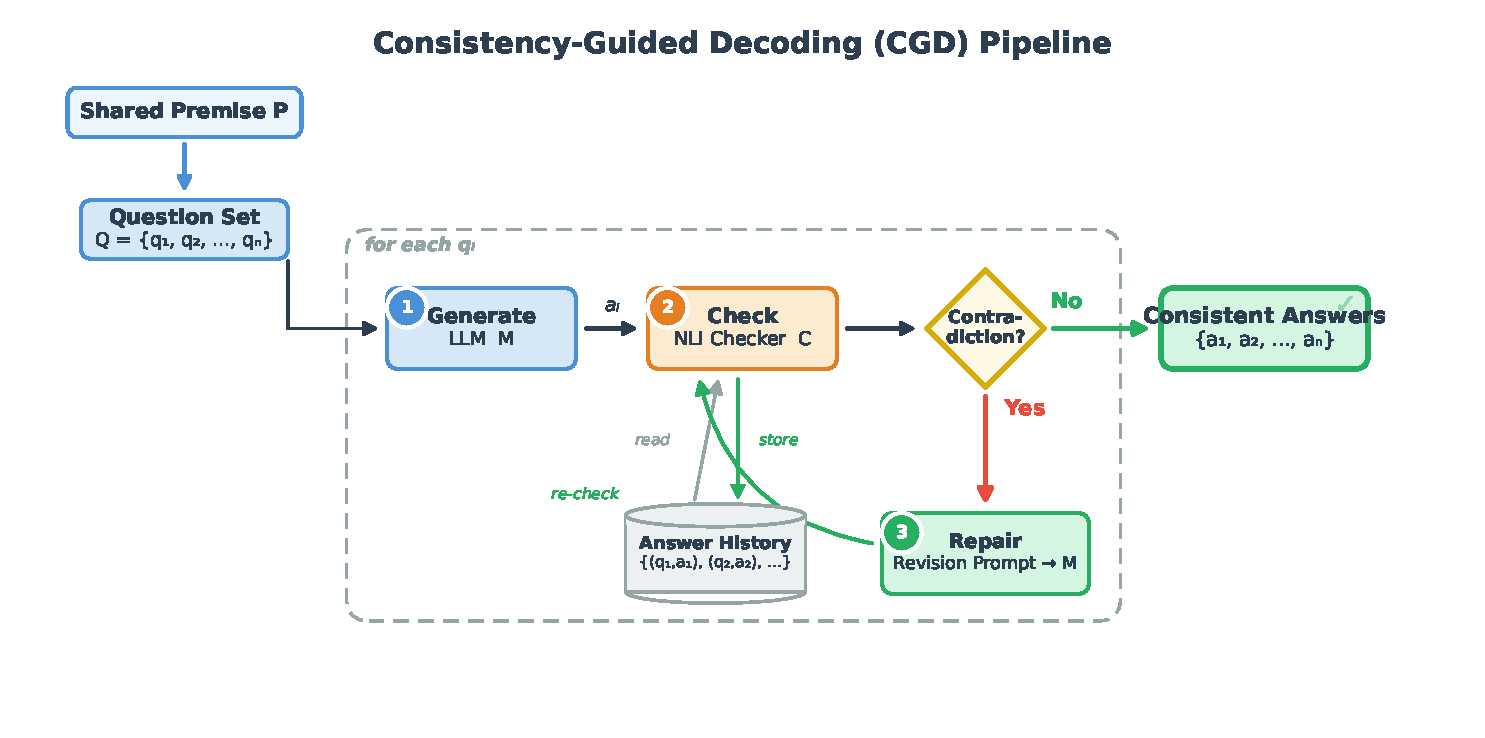
\includegraphics[width=\columnwidth]{figures/cgd_pipeline.pdf}
\caption{\textbf{Consistency-Guided Decoding (\method{}) pipeline.} For each question $q_i$ in a set, the LLM generates an initial answer (Step 1), which is checked against all prior answers in the answer history via an NLI contradiction checker (Step 2). If a contradiction is found, a revision prompt containing the conflicting prior answer and the shared premise is sent back to the LLM (Step 3). The revised answer is then re-checked. Consistent answers are stored in the history for future checks.}
\label{fig:cgd}
\end{figure}

% ============================================================
\section{Full Strategy Comparison}
\label{app:strategies}
% ============================================================

Table~\ref{tab:strategies} provides a detailed comparison across all evaluated strategies (Direct, CoT, \method{}) for models where multiple strategies were tested. The results demonstrate that \method{} outperforms both Direct and CoT prompting on set-level consistency across all models tested with multiple strategies.

\begin{table}[ht]
\caption{Detailed strategy comparison on representative models. CoT = Chain-of-Thought. Bold indicates best result per model per metric.}
\label{tab:strategies}
\begin{center}
\small
\begin{tabular}{llccc}
\toprule
\textbf{Model} & \textbf{Strategy} & \textbf{IA (\%)} & \textbf{PCR (\%)} & \textbf{SCR (\%)} \\
\midrule
\multirow{3}{*}{GPT-4o}
 & Direct & 70.8 & 57.0 & 20.0 \\
 & CoT & 75.0 & 63.5 & 28.3 \\
 & \method{} (Ours) & \textbf{79.0} & \textbf{69.5} & \textbf{39.7} \\
\midrule
\multirow{3}{*}{Qwen 2.5 72B}
 & Direct & 75.0 & 65.0 & 32.7 \\
 & CoT & \textbf{77.1} & 65.3 & 32.3 \\
 & \method{} (Ours) & 73.7 & \textbf{67.8} & \textbf{33.0} \\
\midrule
\multirow{2}{*}{GPT-4.1}
 & Direct & 83.0 & 74.0 & 46.7 \\
 & \method{} (Ours) & \textbf{85.2} & \textbf{77.6} & \textbf{54.0} \\
\midrule
\multirow{2}{*}{GPT-5.2}
 & Direct & 69.3 & 52.3 & 12.0 \\
 & \method{} (Ours) & \textbf{73.2} & \textbf{58.4} & \textbf{23.7} \\
\midrule
\multirow{2}{*}{o3}
 & Direct & 67.2 & 51.8 & 12.0 \\
 & \method{} (Ours) & \textbf{70.3} & \textbf{56.7} & \textbf{21.0} \\
\midrule
\multirow{2}{*}{Cl.\ Sonnet 4.6}
 & Direct & 57.5 & 47.4 & 10.3 \\
 & \method{} (Ours) & \textbf{67.0} & \textbf{57.7} & \textbf{24.3} \\
\bottomrule
\end{tabular}
\end{center}
\end{table}

On GPT-4o, which is the only model evaluated under all three strategies, \method{} achieves 39.7\% SCR compared to 28.3\% for CoT and 20.0\% for Direct prompting, representing a 99\% relative improvement over Direct and a 40\% improvement over CoT. Importantly, \method{} also achieves the highest IA (79.0\%) and PCR (69.5\%) on this model, demonstrating that consistency-aware revision benefits all metrics simultaneously.

For Qwen~2.5 72B, the results reveal an instructive pattern: CoT improves IA from 75.0\% to 77.1\% but slightly \emph{decreases} SCR from 32.7\% to 32.3\%, while \method{} improves SCR to 33.0\%. This illustrates that independent reasoning improvements (CoT) do not automatically translate to cross-query consistency.

% ============================================================
\section{Per-Category SCR Heatmap}
\label{app:category}
% ============================================================

\begin{figure}[ht]
\centering
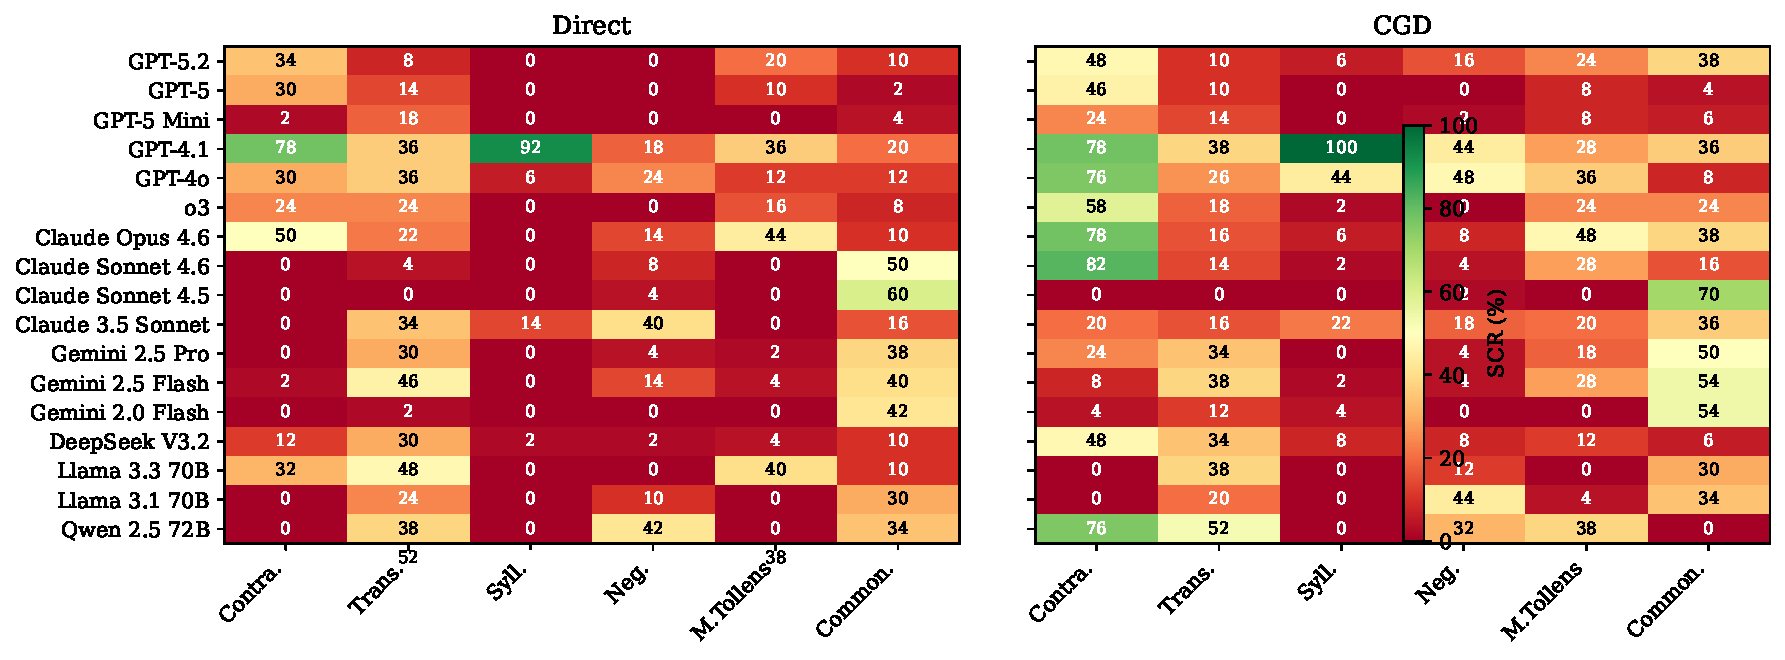
\includegraphics[width=\columnwidth]{figures/category_heatmap.pdf}
\caption{Set-level consistency rate (SCR\%) by category for Direct prompting (left) and \method{} (right) across all evaluated models. \method{} provides improvements across most model-category combinations, with the largest gains on contrapositive and modus tollens categories that specifically test logical equivalence.}
\label{fig:category}
\end{figure}

The heatmap reveals several patterns. Syllogistic reasoning is generally the hardest category, with many models achieving 0\% SCR under Direct prompting. Transitivity and contrapositive categories show moderate scores for the strongest models. Commonsense entailment presents a distinct pattern: some models that perform poorly on formal logic categories achieve relatively higher scores here (e.g., Gemini~2.0 Flash: 42\% commonsense vs.\ 0\% on four formal categories), likely because commonsense reasoning patterns are better represented in pre-training data.

% ============================================================
\section{Consistency Gap Visualization}
\label{app:gap}
% ============================================================

\begin{figure}[ht]
\centering
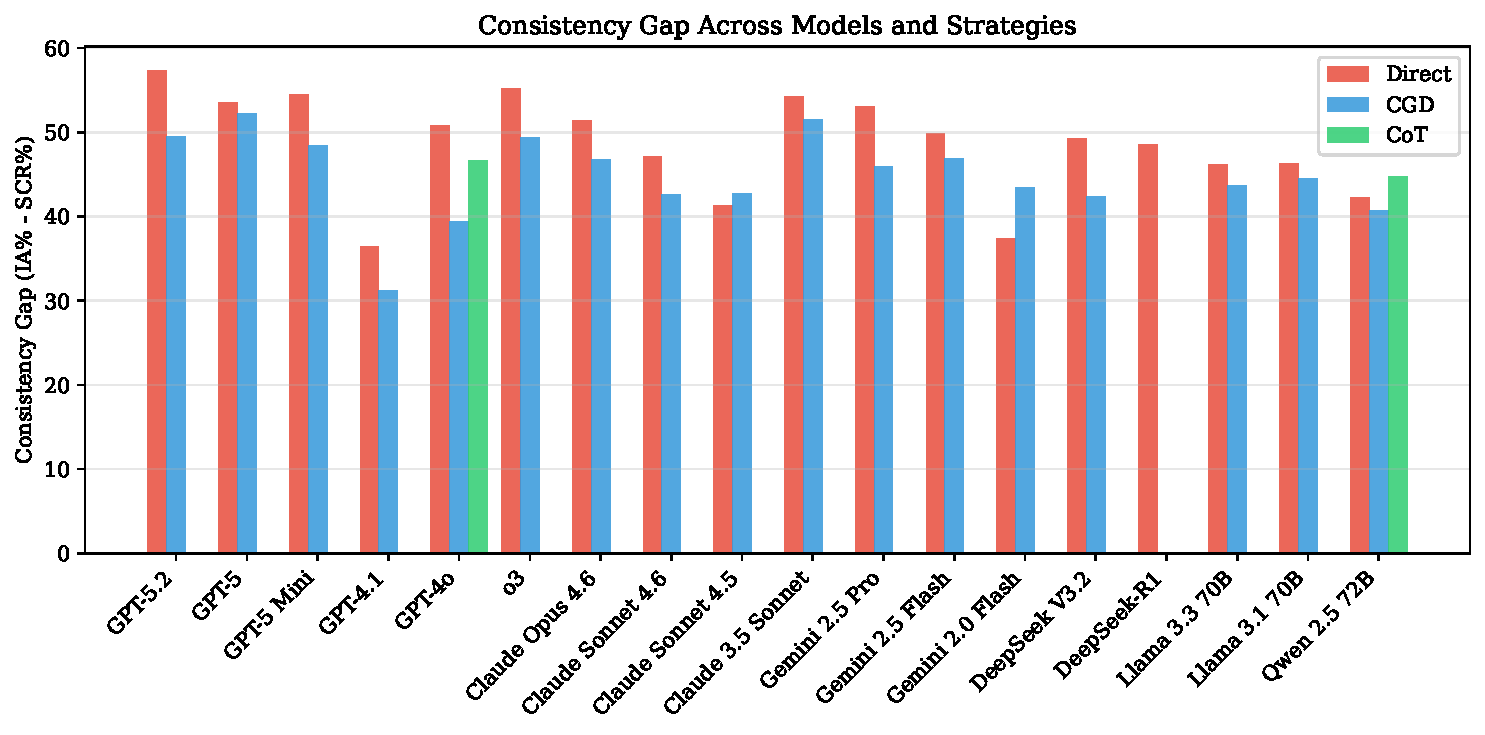
\includegraphics[width=\columnwidth]{figures/consistency_gap.pdf}
\caption{Consistency gap (IA\% $-$ SCR\%) across all models and strategies. Smaller bars indicate better cross-query consistency. \method{} consistently narrows the gap compared to Direct prompting.}
\label{fig:gap}
\end{figure}

The consistency gap visualization reinforces two key findings. First, the gap is \emph{larger} in absolute terms for models with higher IA, because their higher individual accuracy creates more room for SCR to lag behind. For instance, GPT-5.2 has both the highest gap (57.3pp) and a relatively high IA (69.3\%). Second, \method{} reduces the gap primarily by improving SCR more than it changes IA, confirming that the method specifically targets the consistency failure mode rather than broadly improving reasoning.

% ============================================================
\section{Complete Per-Category Breakdown}
\label{app:fullcategory}
% ============================================================

Table~\ref{tab:percategory} provides the complete per-category SCR breakdown for all models evaluated under Direct prompting. Each cell shows the percentage of question sets within that category where the model answered all questions correctly.

\begin{table}[ht]
\caption{Per-category set-level consistency rate (SCR\%) under Direct prompting for select models. Each category has 50 question sets. Values represent the percentage of sets where all questions were answered correctly.}
\label{tab:percategory}
\begin{center}
\small
\setlength{\tabcolsep}{4pt}
\begin{tabular}{l cccccc}
\toprule
\textbf{Model} & \textbf{Contra.} & \textbf{Trans.} & \textbf{Syll.} & \textbf{Neg.} & \textbf{M.Toll.} & \textbf{Comm.} \\
\midrule
GPT-4.1 & 78.0 & 36.0 & 92.0 & 18.0 & 36.0 & 20.0 \\
Qwen 2.5 72B & 78.0 & 52.0 & 0.0 & 28.0 & 38.0 & 0.0 \\
Cl.\ Opus 4.6 & 50.0 & 22.0 & 0.0 & 14.0 & 44.0 & 10.0 \\
GPT-4o & 30.0 & 36.0 & 6.0 & 24.0 & 12.0 & 12.0 \\
GPT-5.2 & 34.0 & 8.0 & 0.0 & 0.0 & 20.0 & 10.0 \\
o3 & 24.0 & 24.0 & 0.0 & 0.0 & 16.0 & 8.0 \\
Gemini 2.0 Flash & 0.0 & 2.0 & 0.0 & 0.0 & 0.0 & 42.0 \\
\bottomrule
\end{tabular}
\end{center}
\end{table}

Several patterns emerge from this breakdown. GPT-4.1 achieves an exceptional 92\% on syllogistic reasoning, far above all other models, yet scores only 18\% on negation and 20\% on commonsense entailment. Qwen~2.5 72B shows an extreme pattern: 78\% on contrapositive and 52\% on transitivity, but exactly 0\% on syllogistic and commonsense. This highly uneven performance across categories suggests that models acquire logical patterns idiosyncratically rather than developing general logical competence. Gemini~2.0 Flash presents a particularly striking case: it achieves 0\% SCR on four of six formal categories but 42\% on commonsense entailment, suggesting that its performance is driven by surface pattern matching on commonsense patterns rather than logical reasoning.

% ============================================================
\section{Qualitative Error Analysis}
\label{app:errors}
% ============================================================

Table~\ref{tab:errors} shows representative examples of cross-query contradictions from the Direct prompting evaluation.

\begin{table}[t]
\caption{Representative cross-query contradictions. The model answers Q1 correctly but contradicts itself on Q2, despite Q2 being logically entailed by the same premises.}
\label{tab:errors}
\begin{center}
\small
\begin{tabular}{p{1.2cm}p{5.5cm}p{1cm}p{1cm}}
\toprule
\textbf{Category} & \textbf{Question (abbreviated)} & \textbf{Exp.} & \textbf{Pred.} \\
\midrule
Common. & Q1: Given that "The election results were announced", is it reasonable to conclude t... & Yes & Yes \\
         & Q2: If we know that it is NOT the case that "an election took place", is it possible... & No & N/A \\
\midrule
Neg. & Q1: Is the following statement true? "Gravity pulls objects toward the center of the... & Yes & Yes \\
         & Q2: Is the negation of the following statement true? "It is NOT the case that gravit... & No & Yes \\
\midrule
M.Tollens & Q1: Given: "If the road is clear, then Victor goes for a walk." We observe that Vict... & Yes & Yes \\
         & Q2: Given: "If the road is clear, then Victor goes for a walk." We observe that Vict... & No & No \\
\midrule
\bottomrule
\end{tabular}
\end{center}
\end{table}

\paragraph{Common error patterns.}
We identify three dominant error patterns:
\begin{enumerate}
    \item \textbf{Contrapositive blindness} (most common): Models affirm $P \to Q$ but deny $\neg Q \to \neg P$, treating the contrapositive as a separate and uncertain claim rather than a logical equivalence.
    \item \textbf{Fallacy acceptance}: Models frequently affirm the consequent (``Q is true, therefore P is true'') and deny the antecedent (``not P, therefore not Q''), treating these invalid inferences as valid.
    \item \textbf{Over-cautious hedging}: On some questions, models output ``Cannot be determined'' when the answer is logically certain, particularly for contrapositive and transitive inferences.
\end{enumerate}

\paragraph{\method{} repair examples.}
When \method{} detects a contradiction (e.g., answering ``No'' to the contrapositive after answering ``Yes'' to modus ponens), the revision prompt surfaces the inconsistency. In the majority of cases, the model corrects itself when shown the contradiction, suggesting that the knowledge of logical equivalence is latent but not reliably activated during independent generation.

% ============================================================
\section{Full Benchmark Statistics}
\label{app:benchmark}
% ============================================================

\bench{} contains 493 question sets with 1,904 individual questions. The benchmark is designed for measuring cross-query logical consistency and tests six categories of reasoning. Table~\ref{tab:benchstats} summarizes the benchmark statistics.

\begin{table}[ht]
\caption{Full \bench{} statistics. The evaluation sample uses a stratified subset of 300 sets (50 per category).}
\label{tab:benchstats}
\begin{center}
\small
\begin{tabular}{lc}
\toprule
\textbf{Statistic} & \textbf{Value} \\
\midrule
Total question sets & 493 \\
Total individual questions & 1,904 \\
Questions per set & 3--4 \\
Number of categories & 6 \\
Sets per formal category & 85 \\
Sets in commonsense category & 68 \\
\midrule
Evaluation sample: sets & 300 \\
Evaluation sample: questions & 1,150 \\
Sets per category (eval) & 50 \\
\midrule
Entity pools: person names & 24 \\
Entity pools: factual statements & 20 \\
Entity pools: activity pairs & 10 \\
Entity pools: condition pairs & 8 \\
Entity pools: abstract categories & 10 \\
Entity pools: commonsense rules & 70 \\
\midrule
Total models evaluated & 18 \\
Total evaluation runs & 37 \\
Models with Direct results & 18 \\
Models with CGD results & 17 \\
Models with CoT results & 2 \\
\bottomrule
\end{tabular}
\end{center}
\end{table}

Questions are generated programmatically from curated entity pools. For formal categories, the premise structure follows classical logic (e.g., ``If $P$ then $Q$'') and questions test the direct inference, contrapositive, converse, and inverse. For commonsense entailment, premises describe everyday situations (e.g., ``The election results were announced'') and questions test whether the model correctly identifies entailed conclusions and rejects non-entailed ones. All ground-truth labels are verified by the authors.

% ============================================================
\section{Prompting Templates}
\label{app:prompts}
% ============================================================

We use three prompting strategies across our evaluation. The exact system prompts and formatting templates are reproduced below.

\paragraph{Direct (vanilla) prompting.}
\begin{quote}
\small
\textit{System}: You are a precise logical reasoning assistant. Answer questions based strictly on the given premises and logical rules. Be concise and clear. Always start your final answer with one of: ``Yes'', ``No'', or ``Cannot be determined''.

\textit{User}: Premise: [premise text]

Question: [question text]
\end{quote}

\paragraph{Chain-of-Thought (CoT) prompting.}
\begin{quote}
\small
\textit{System}: You are a precise logical reasoning assistant. Think step by step through the logical reasoning before giving your final answer. State your final answer starting with ``FINAL ANSWER:'' followed by ``Yes'', ``No'', or ``Cannot be determined''.

\textit{User}: Premise: [premise text]

Question: [question text]

Think through this step by step:
\end{quote}

\paragraph{\method{} NLI contradiction check.}
\begin{quote}
\small
\textit{System}: You are a logical consistency checker. Given two statements derived from the same premise, determine if they contradict each other. Answer ``CONTRADICTION'' or ``NO CONTRADICTION'' only.

\textit{User}: Premise: [shared premise]

Statement 1 (prior answer): [prior question] $\rightarrow$ [prior answer]

Statement 2 (current answer): [current question] $\rightarrow$ [current answer]

Do these two answers contradict each other given the shared premise?
\end{quote}

\paragraph{\method{} revision prompt.}
\begin{quote}
\small
\textit{User}: You previously answered a related question as follows:

Question: [prior question]

Your answer: [prior answer]

However, your current answer to the following question may be logically inconsistent with your previous answer:

Current question: [current question]

The logical relationship is based on this shared premise: [shared premise]

Please reconsider your answer to the current question, ensuring logical consistency with your previous answer. Start your final answer with ``Yes'', ``No'', or ``Cannot be determined''.
\end{quote}

% ============================================================
\section{Per-Model Family Analysis}
\label{app:families}
% ============================================================

Table~\ref{tab:families} summarizes the results by model family, showing that the consistency gap is a cross-family phenomenon.

\begin{table}[ht]
\caption{Results aggregated by model family. Values show the range (min--max) across models within each family for Direct prompting.}
\label{tab:families}
\begin{center}
\small
\begin{tabular}{l c c c c}
\toprule
\textbf{Family} & \textbf{\#Models} & \textbf{IA Range} & \textbf{SCR Range} & \textbf{Gap Range} \\
\midrule
OpenAI & 6 & 58.4--83.0 & 4.0--46.7 & 36.4--57.3 \\
Anthropic & 4 & 51.9--74.8 & 10.3--23.3 & 41.2--54.2 \\
Google & 3 & 44.7--67.6 & 7.3--17.7 & 37.4--53.1 \\
DeepSeek & 2 & 59.2--70.2 & 10.0--21.7 & 48.5--49.2 \\
Meta (Llama) & 2 & 56.8--65.3 & 10.7--19.0 & 46.1--46.3 \\
Qwen & 1 & 75.0 & 32.7 & 42.3 \\
\midrule
\textbf{All} & \textbf{18} & 44.7--83.0 & 4.0--46.7 & 36.4--57.3 \\
\bottomrule
\end{tabular}
\end{center}
\end{table}

\paragraph{OpenAI family.} The OpenAI models show the widest performance range. GPT-4.1 is the clear best performer overall (SCR 46.7\%), while GPT-5 Mini is the weakest in the entire evaluation (SCR 4.0\%). Notably, the newer GPT-5 series models (GPT-5.2: 12.0\%, GPT-5: 9.3\%, GPT-5 Mini: 4.0\%) perform substantially \emph{worse} on consistency than the older GPT-4.1 (46.7\%), despite likely having higher general capability. The reasoning-specialized o3 (12.0\%) does not outperform GPT-4.1 on consistency. Under \method{}, GPT-4o shows the largest improvement of any model (+19.7pp), reaching 39.7\% SCR.

\paragraph{Anthropic family.} Claude Opus~4.6 leads the Anthropic family with 23.3\% SCR under Direct prompting and benefits substantially from \method{} (+9.0pp to 32.3\%). Claude Sonnet~4.6 shows an interesting pattern: relatively low vanilla SCR (10.3\%) but one of the largest \method{} improvements (+14.0pp to 24.3\%), suggesting particularly strong latent consistency knowledge that is activated by the revision mechanism.

\paragraph{Google family.} The Gemini models show moderate IA but low SCR. Gemini~2.0 Flash has the lowest IA in the evaluation (44.7\%) but benefits from \method{} with the largest IA improvement of any model (+11.0pp), suggesting that the contradiction-aware revision helps this model avoid systematic errors.

\paragraph{DeepSeek family.} DeepSeek-R1, a reasoning-specialized model, achieves a respectable 21.7\% SCR, outperforming most models despite being designed primarily for extended reasoning chains rather than cross-query consistency. DeepSeek V3.2 benefits substantially from \method{} (+9.3pp).

\paragraph{Meta and Qwen.} The Llama models show moderate performance. Llama~3.1 70B is the only model where \method{} hurts ($-$2.0pp), possibly because the model's limited reasoning capacity leads to error propagation during revision. Qwen~2.5 72B achieves the second-best vanilla SCR (32.7\%) and shows minimal but positive improvement with \method{} (+0.3pp), suggesting that this model's consistency is already relatively well-calibrated.

% ============================================================
\section{Summary of CGD Improvements}
\label{app:cgdsummary}
% ============================================================

\begin{table}[ht]
\caption{Summary statistics for \method{} improvements across 17 models.}
\label{tab:cgdsummary}
\begin{center}
\small
\begin{tabular}{lcc}
\toprule
\textbf{Metric} & \textbf{$\Delta$SCR} & \textbf{$\Delta$IA} \\
\midrule
Mean & +6.6pp & +2.8pp \\
Median & +5.0pp & +2.3pp \\
Max & +19.7pp (GPT-4o) & +11.0pp (Gem.\ 2.0 Flash) \\
Min & $-$2.0pp (Llama 3.1 70B) & $-$3.7pp (Llama 3.1 70B) \\
Models improved (SCR) & 16 / 17 (94\%) & 13 / 17 (76\%) \\
Models improved (IA) & 13 / 17 & -- \\
\bottomrule
\end{tabular}
\end{center}
\end{table}

The improvement distribution is right-skewed: four models gain more than +9pp SCR (GPT-4o, Claude Sonnet~4.6, GPT-5.2, and tied at +9.0pp: Claude Opus~4.6 and o3), while five models gain less than +3pp. This suggests that \method{} is most effective for models that have strong individual reasoning capability but fail to apply it consistently across queries, a condition met by most frontier models.

% ============================================================
\section{Reproducibility Details}
\label{app:reproducibility}
% ============================================================

All models were accessed via their respective commercial APIs between January and February 2026. We used temperature 0 (or the minimum available temperature) for all evaluations to ensure deterministic outputs. The NLI contradiction checker in \method{} uses GPT-4o-mini with temperature 0. Evaluation scripts are implemented in Python and process each question set sequentially. Answer extraction uses exact-match parsing of the first word (``Yes'', ``No'', or ``Cannot be determined'') from the model's response.

The total evaluation cost was approximately \$105 across all 37 evaluation runs (18 models $\times$ Direct + 17 $\times$ \method{} + 2 $\times$ CoT), using OpenRouter API credits. \method{} runs cost approximately 1.5$\times$ the corresponding Direct run due to the additional NLI checks and occasional revision prompts.

\end{document}
